\subsection{Description of the model}
\label{sec:Description}


%description of the model - components and functions
We describe here a system-level model implemented to explain the hypothesis that intrinsiclly generated goals guide learning at the very first stages of sensorimotor development. 
%
The model is made of several interacting functional components.  
%
A first component, the goal generator (GC), implements the unsupervised generation of internal categories of sensory inputs. These categories will be used in the model as abstract representations of the world that can be targeted as goals. The GC takes information from touch sensors distributed all over the body of the agent (see below). This information is filtered so that only somatosensory increments are retained. This information about sensory saliency is further transformed so that it results in a two-dimensional retina composed of horizontally-distributed receptive fields. Figure~\ref{fig:sensory-input} shows this process. The one-dimentional body space of the agent (two arms and a line-shaped torso) is converted in a two-dimensonal touch retina. 

\begin{figure}[htp]
\centering
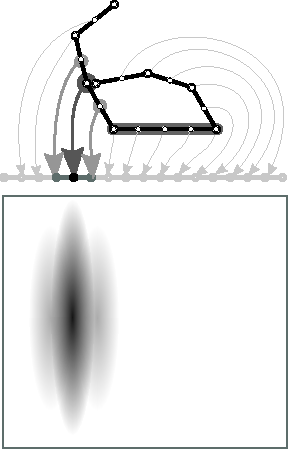
\includegraphics[scale=1.0]{sensoryinput}
\caption{}
\label{fig:sensory-input}
\end{figure}


 In the current implementatiion the GC is  a self organizing map (SOM).   

The model is based on five components: (1) a competitive neural network, supporting the acquisition of abstract representations based on experienced changes in the sensory input; (2) a selector that on the basis on competence-based intrinsic motivations (CB-IMs) determines the pursued goal and which motor resources will be trained to obtain that goal; (3) an echo-state neural network that controls the movements of the robot and supports the acquisition of the motor skills; (4) a predictor of the accomplishment of the pursued goal, used to measure the improvement of the system competence; (5) the generator of the CB-IM signal that biases the activity of the selector.
 
\subsection{Implementation details}
\label{sec:Implementation}

\subsection{Setup}
\label{sec:Setup}